\documentclass[12pt]{article}
\usepackage[a4paper, left=2.0cm,top=2.0cm,right=1.0cm,bottom=2.0cm]{geometry}
\usepackage[utf8]{inputenc}
\usepackage[portuguese]{babel}
\usepackage{graphicx}
\usepackage{float}
\usepackage{lmodern}
\usepackage{hyperref}
\usepackage{amsmath}
\usepackage{amsfonts}
\usepackage{multicol}
\usepackage{gensymb}
\usepackage{amssymb}
\usepackage[dvipsnames]{xcolor}
\usepackage{multirow} %para multiplas linhas (merge)
\usepackage{colortbl} %colorir célula
\usepackage{array} %redimensionar tabela
\usepackage{tabularx} % definição do redimensionamento
\usepackage{wrapfig}

\begin{document}

\begin{tabular}{lllll}
\multirow{3}*{
\includegraphics[width=90px]{2.jpg}}
&\multicolumn{4}{l}{ESCOLA CASTRO ALVES E JI MORAGUINHO} \multirow{3}*{
\includegraphics[width=90px]{1.jpg}}\\
& CAXIAS, \underline{\hspace{0.7cm}}\,DE \underline{\hspace{2cm}} \,DE 2021&  & \\ 
& ALUNO(A): \underline{\hspace{6.8cm}}&  & \\ 
& SÉRIE: PRÉ-VESTIBULAR TURMA: A ( )  B ( )   & & \\
& TURNO: \underline{\hspace{2.5cm}} PROFº:  ROBERT MELO &  & \\
\end{tabular} \bigskip

\begin{center}

ATIVIDADE DE FÍSICA I

\end{center}
%
\begin{multicols}{2}
%
\begin{enumerate}
\item A canoagem de velocidade ganhou status de modalidade olímpica em 1936. Suas provas ocorrem em locais de águas calmas e percursos de 200, 500 e 1.000 metros e podem ser disputadas em categorias de canoa ou kayak.
\\
\\
Considerando que a prova de canoagem seja realizada a favor da correnteza, a representação do deslocamento (s) e da velocidade (v) da canoa em relação ao tempo (t) está indicada
em

\begin{figure}[!h]
    %\caption{Circuito Elétrico} %legenda
    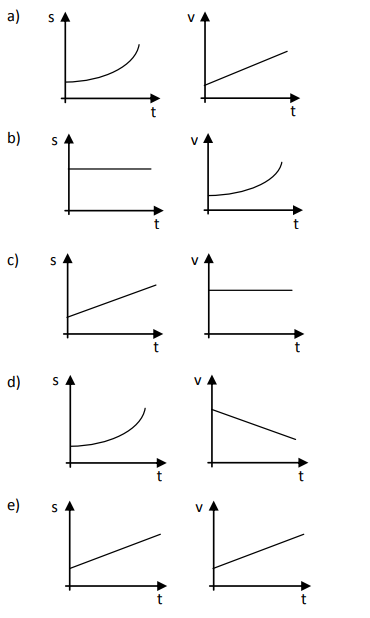
\includegraphics[width=1cm]{10} %endereço da imagem
    \label{fig:my_label} %marcador
\end{figure}

\end{enumerate}

\end{multicols}

\end{document}